\textbf{\underline{OZ 7 - Inductantie - Oefening 1:}}
\vspace{0.5cm}

Bepaal voor de toroïde de energiedichtheid in het magnetisch veld in
functie van $r$ waarbij $r_1 < r < r_2$. Integreer dit over het volume om de totale energie
opgeslagen in de toroïde te vinden. De toroïde bevat $N$ windingen en draagt een
stroom $I$.

\begin{center}
    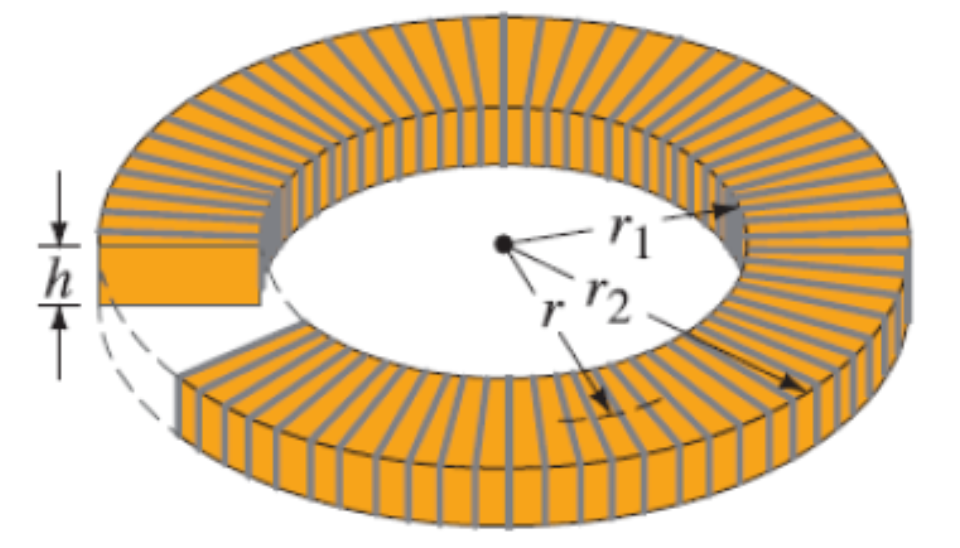
\includegraphics[scale = 0.3]{oz07/resources/Oz7Oef1.png}
\end{center}

\begin{description}[labelwidth=1.5cm, leftmargin=!]
    \item[Geg. :] 
    \item[Gevr. :] 
    \item[Opl. :]
\end{description}

\vspace{1cm}